%%%%%%%%%%%%%%%%%%%%%%%%%%%%%%%%%%%%%%%%%%%%%%%%%%%%%%%%%%%%%%%%%%%%%%%%%%%
%%  chapter5.tex  –  Глава 5: Программная платформа RobustIDPS.ai
%%  v9 – Глава промышленного развёртывания: целевые пользователи, 46-стр. PWA,
%%       10 функциональных групп, 17 моделей, защита LLM, PQC-IDS,
%%       плагин Snort/Suricata, 8 рисунков для скриншотов.
%%       Только заголовки \section добавлены в оглавление.
%%%%%%%%%%%%%%%%%%%%%%%%%%%%%%%%%%%%%%%%%%%%%%%%%%%%%%%%%%%%%%%%%%%%%%%%%%%

\chapter{Система анализа сетевого трафика на основе программной платформы RobustIDPS.ai}
\label{ch:platform}

В настоящей главе систематически представлена программная
\emph{система} \textsf{RobustIDPS.ai}~\cite{Anaedevha2026robustidps}
(DOI:~\url{10.5281/zenodo.19129512}; исходный код:
\url{https://github.com/rogerpanel/robustidps.ai}), реализующая
семёрку гибридная СОПВ из \S\ref{sec:hybrid_idps_math_model}
применительно к сектору защиты сетевого трафика. Структура главы
следует трёхзвенной схеме, заданной указанием научного руководителя:
\emph{(I)~постановка задачи} формализует входы, выходы и режим
работы системы для рассматриваемого сектора
(\S\ref{sec:platform_problem_statement}); \emph{(II)~описание
системы / программной реализации} систематически охватывает
варианты использования, функциональность, документацию, реализацию
фронтенда и бэкенда, двухплоскостную архитектуру (Python-плоскость
управления + Rust-плоскость данных, релиз~v4), функциональные
группы (51~страница в 10~группах), 17~интегрированных моделей
обнаружения, миграцию граничного агента на Rust с ядерно-резидентным
быстрым путём XDP и операционную инфраструктуру развёртывания
(\S\ref{ch:platform}--\S\ref{sec:deployment});
\emph{(III)~апробация системы} систематически документирует
результаты валидации, сравнение с коммерческими и открытыми
платформами, вклад в открытый исходный код и акты внедрения от
профильных организаций
(\S\ref{sec:platform_comparison}--\S\ref{sec:opensource}).
Включены не менее шести скриншотов пользовательского интерфейса
системы для иллюстрации её операционных возможностей.

Глава содержит исчерпывающее описание программной системы как
прямое инстанцирование математической модели гибридной СОПВ,
сформулированной в Главе~\ref{ch:methods}: каждый из семи методов
(М1--М7) отображается на конкретный программный компонент с
явными API-интерфейсами и операционными метриками. Архитектурно
платформа реализует принципы безопасной разработки <<security by
design>>, включая мульти-тенантную ролевую модель доступа (RBAC),
полное журналирование действий пользователей через
структурированные логи, защищённое хранение чувствительных
конфигурационных параметров через интеграцию с HashiCorp Vault и
строгую сегментацию между плоскостями управления и данных,
описанную в~\S\ref{sec:platform_problem_statement}. Этот подход
обеспечивает прослеживаемость от математических теорем к
работающему коду с минимальным разрывом абстракции и позволяет
независимым разработчикам и интеграторам безопасности воспроизвести
заявленные показатели качества, робастности и эффективности на
собственной инфраструктуре. В дополнение к опубликованному
исходному коду (Zenodo, DOI:~\url{10.5281/zenodo.19129512})
платформа сопровождается полной технической документацией,
наборами демонстрационных данных и сценариями автоматизированного
тестирования, что снижает порог входа для академических
исследовательских групп и промышленных команд кибербезопасности.

%%=====================================================================\section{Организация опытной эксплуатации системы}
\label{sec:platform_problem_statement}%%=====================================================================

Задача защиты сетевого трафика рассматривается в настоящей главе как
конкретная инстанцированная задача семёрки гибридная СОПВ из
\S\ref{sec:hybrid_idps_math_model}. Формально, на вход системы
поступает поток сетевых пакетов (PCAP, NetFlow, EVE~JSON) и
оповещений сигнатурных движков (Snort, Suricata), агрегированных
конвейером преобразования данных в граф из
Главы~\ref{ch:adaptation}; на выходе система формирует
ранжированные оповещения, развёртываемые правила Snort/Suricata,
а также управляющие действия активного реагирования (блокировка
потока, изоляция узла, эскалация в SIEM/SOAR). Высокоуровневая
схема приведена на рис.~\ref{fig:platform_problem_box}.

\textsf{RobustIDPS.ai}~--- комплексная ИИ-нативная платформа
обнаружения и предотвращения вторжений, содержащая 51 взаимосвязанную
страницу, организованную в 10 функциональных групп, интегрирующая 17
моделей машинного и глубокого обучения для классификации сетевого
трафика по 34 классам атак и 83 инженерным признакам. Платформа
решает три ограничения существующих коммерческих аналогов
(CrowdStrike Charlotte AI, SentinelOne Purple AI, Microsoft Security
Copilot, Google Sec-Gemini~\cite{Smith2023}): проприетарная
интеграция LLM одного вендора, препятствующая межпровайдерному
бенчмаркингу, отсутствие систематической оценки состязательной
робастности и отсутствие поддержки анализа постквантового
криптографического трафика. Платформа предназначена для пяти
категорий целевых пользователей: SOC-аналитиков (Уровни 1--3),
инженеров кибербезопасности, исследователей MLSecOps, разработчиков
ИИ и академических исследователей в области робастности графовых
нейронных сетей.

\noindent\textbf{Технологический стек.} \textsf{RobustIDPS.ai}
развёрнута как прогрессивное веб-приложение (PWA) со следующим
стеком, выбранным для обеспечения одновременно: \emph{(i)}~
воспроизводимого обучения и инференса глубоких графовых
нейросетевых моделей М1--М7; \emph{(ii)}~устойчивой потоковой
обработки сетевого трафика в режиме реального времени;
\emph{(iii)}~интерактивного пользовательского интерфейса аналитика
SOC; и \emph{(iv)}~интеграции с внешними поставщиками больших
языковых моделей (LLM) через единый API-абстрактный слой.
\emph{Фронтенд}~--- одностраничное приложение React~18 с
компонентами Material-UI, адаптивным дизайном и манифестом PWA для
развёртывания с поддержкой офлайн-режима через кэширование
сервис-воркером; \emph{бэкенд}~--- Flask/Python~3.11+ с 60+ RESTful
API эндпоинтами, постоянными WebSocket-каналами для мониторинга в
реальном времени и Celery для асинхронного выполнения задач
(обучение моделей, пакетный анализ); \emph{слой данных}~---
PostgreSQL~16 для реляционного хранения (профили пользователей,
журналы обнаружений, записи расследований), Redis~7 для кэширования
и управления сессиями, файловое хранилище для загруженных PCAP/CSV
наборов данных; \emph{оркестрация}~--- Docker Compose обеспечивает
развёртывание одной командой с конфигурацией на основе переменных
окружения для профилей разработки, промежуточного этапа и
производства.

\noindent\textbf{Двухплоскостная архитектура (релиз~v4).} В
релизе~v4 введено чёткое разделение между \emph{плоскостью
управления} (существующий Python-бэкенд на FastAPI,
мультитенантный RBAC, аудит, маршрутизатор LLM) и новой
\emph{плоскостью данных} в виде нативных Rust-агентов,
развёртываемых рядом или перед плоскостью управления. Это
архитектурное решение обусловлено тремя соображениями:
\emph{(а)}~Python-плоскость управления отличается богатым
функционалом и интерактивностью, но её GIL и интерпретируемость
ограничивают пропускную способность на уровне сотен тысяч
потоков/с; \emph{(б)}~Rust обеспечивает память-безопасность без
сборщика мусора и предоставляет нулевую стоимость абстракций для
критических путей обработки трафика; \emph{(в)}~XDP-режим
работы в ядре Linux обеспечивает обработку пакетов до
аллокации \texttt{sk\_buff}, что недостижимо в пользовательском
пространстве независимо от используемого языка. Плоскости
общаются по gRPC. Плоскость данных состоит из двух компонентов:
\texttt{robustidps-edge}~--- долгоживущий gRPC-демон с горячей
подменой ONNX-моделей и потоковой передачей записей о потоках в
плоскость управления; \texttt{robustidps-xdp}~--- LPM-trie блок-лист
в ядре, подключённый через хук XDP в режиме \texttt{Native} на
интерфейсе \texttt{eth0}, обеспечивающий микросекундные решения о
сбросе пакетов. Тем самым достигается одновременно богатое
пользовательское UX в Python-плоскости и режим \emph{wire-speed}
в плоскости данных без каких-либо изменений в существующих 51
страницах фронтенда.

\begin{figure}[htbp]
\centering
\begin{tikzpicture}[font=\scriptsize,
  inp/.style={draw,rounded corners=2pt,fill=blue!10,
    minimum width=3.0cm,minimum height=11mm,align=center,thick},
  sys/.style={draw,rounded corners=3pt,fill=orange!18,
    minimum width=5.0cm,minimum height=22mm,align=center,
    font=\small\bfseries,thick,draw=orange!70!black},
  outbx/.style={draw,rounded corners=2pt,fill=green!12,
    minimum width=3.0cm,minimum height=11mm,align=center,thick,
    draw=green!55!black},
  arr/.style={-{Stealth[length=2.5mm]},semithick,gray!75!black,thick}]
\node[inp] (in1) {Поток сетевых\\пакетов / NetFlow};
\node[inp,below=4mm of in1] (in2) {События сигнатурных\\движков Snort/Suricata};
\node[sys,right=22mm of $(in1)!0.5!(in2)$] (sys)
  {Система\\гибридная СОПВ\\\textsf{RobustIDPS.ai}\\\scriptsize 17 моделей М1--М7};
\node[outbx,right=22mm of sys.north east,yshift=0mm,anchor=west] (out1)
  {Ранжированные\\оповещения};
\node[outbx,right=22mm of sys.east,anchor=west] (out2)
  {Правила Snort/\\Suricata};
\node[outbx,right=22mm of sys.south east,anchor=west] (out3)
  {Активные\\действия (SOAR)};
\draw[arr] (in1) -- (sys.north west);
\draw[arr] (in2) -- (sys.south west);
\draw[arr] (sys.north east) -- (out1);
\draw[arr] (sys.east) -- (out2);
\draw[arr] (sys.south east) -- (out3);
\end{tikzpicture}
\caption{Постановка задачи защиты сетевого трафика системой
гибридная СОПВ в реализации платформы~\textsf{RobustIDPS.ai}. Слева~---
входные потоки (сетевые пакеты, NetFlow, оповещения сигнатурных
движков); в центре~--- система с 17~интегрированными моделями
М1--М7; справа~--- выходные артефакты (ранжированные оповещения,
развёртываемые правила Snort/Suricata, управляющие действия для
SIEM/SOAR-оркестрации).}
\label{fig:platform_problem_box}
\end{figure}

\noindent\textbf{Целевые свойства системы в данном секторе.}
Решение задачи защиты сетевого трафика
системой~\textsf{RobustIDPS.ai} систематически удовлетворяет
четырём из шести свойств~П1--П6 из~\S\ref{subsec:six_properties}:
\emph{П1} (состязательная устойчивость, ур.~\eqref{eq:adv_resilient_property})
обеспечивается интеграцией методов~М1, М4 и~М7;
\emph{П2} (робастность, ур.~\eqref{eq:robustness_property})
подтверждается результатами Главы~\ref{ch:adaptation}
(\S\ref{sec:method_results});
\emph{П3} (эффективность, ур.~\eqref{eq:efficiency_property})
обеспечивается двухплоскостной архитектурой~v4 с ядерно-резидентным
быстрым путём XDP (\S\ref{ch:platform});
\emph{П5} (человеческий фактор, ур.~\eqref{eq:calibration_property})
реализуется через сортировку оповещений по неопределённости в
SOC-копилоте (\S\ref{ch:platform}).

%%=====================================================================
%%   ЧАСТЬ II: ОПИСАНИЕ СИСТЕМЫ / ПРОГРАММНАЯ РЕАЛИЗАЦИЯ
%%   (систематически охватывает §§5.2--5.12 ниже:
%%    варианты использования, функциональность, документация,
%%    фронтенд/бэкенд, архитектура, модели, развёртывание)
%%=====================================================================

%%=====================================================================\section{Интеграция системы с существующими средствами защиты информации}
\label{sec:deployment}%%=====================================================================

RobustIDPS.ai предназначена для развёртывания как плагин для существующих систем обнаружения вторжений, в частности Snort~3~\cite{Roesch1999} и Suricata. Архитектурная цель интеграции~--- сохранить уже сделанные организацией инвестиции в сигнатурный контур безопасности, дополнив его ML-нативным слоем без необходимости замены существующих инструментов. Это снижает затраты на внедрение, упрощает прохождение внутренних аудитов и обеспечивает обратную совместимость с существующими процедурами реагирования на инциденты. Интеграция работает через два механизма:

\noindent\textbf{Активная защита ИИ.} Группа активной защиты ИИ
содержит пять страниц, поддерживающих проактивные сценарии
кибербезопасности. \emph{Арена красной команды} обеспечивает
интерактивную среду для проведения состязательных атак на
работающие модели обнаружения с шестью семействами атак (FGSM,
PGD, C\&W, DeepFool, HopSkipJump, BoundaryAttack), позволяя
исследователям и тестировщикам проверять устойчивость своих
обученных моделей до развёртывания. \emph{Реагирование на угрозы}
автоматизирует генерацию управляющих действий через интеграцию
с SOAR-системами (Phantom, Demisto, IBM Resilient).
\emph{SOC-копилот} (наследник наработок Microsoft Security Copilot,
но открытый и мультипровайдерный) обеспечивает
эпистемически-направленную сортировку оповещений на основе UC-HGP
из метода~М6. \emph{Федеративное обучение} реализует
визант-устойчивую агрегацию (FedLLM-API из метода~М2) с
поддержкой до 50~участников и формальной
$(\varepsilon{=}0{,}85,\delta{=}10^{-5})$-дифференциальной
приватностью. \emph{Предиктор цепочек атак} прогнозирует
наиболее вероятные следующие шаги нарушителя на основе
наблюдаемых ранних индикаторов компрометации, используя
теоретико-игровую сертификацию из метода~М7.

\noindent\textbf{Поверхности атак LLM.} Шесть страниц этой группы
систематически охватывают поверхности атак на работающие
LLM-компоненты внутри инфраструктуры безопасности~--- область,
не охватываемая ни одной из существующих коммерческих
платформ. Помимо описанных выше пяти модулей (инъекция промптов,
джейлбрейки, отравление RAG, мультиагентная цепочка, отравление
данных), шестая страница~--- \textsf{MambaGuard}~--- представляет
протоколо-осведомлённый детектор для четырёх протоколов
LLM-агентов: MCP (Model Context Protocol от Anthropic), ACP
(Agent Communication Protocol от Google), A2A (Agent-to-Agent
Protocol от Microsoft) и ANP (Agentic Network Protocol).
\textsf{MambaGuard} достигает макроусреднённого F1=0,978 на
собственном наборе данных MambaGuard-bench при времени инференса
1,8\,мс/поток. Сертификация ансамбля защиты использует
рандомизированное сглаживание для непрерывных бюджетов
возмущений, конформный байесовский интервал для калибровки
вероятностных выходов и регрет-сертификат для онлайн-агентных
сценариев. Группа также интегрирована с панелью соответствия
OWASP LLM Top~10 (2025) с автоматическим картированием каждого
обнаружения в соответствующую категорию риска.

\noindent\textbf{Возможности страниц <<Командного центра ИИ>>.}
Командный центр ИИ~--- основной операционный интерфейс, включающий
пять страниц для сквозного анализа трафика от загрузки до
разрешения оповещений. \emph{Основная панель} отображает
статистику обнаружения в реальном времени: общее число
проанализированных потоков, распределение атак по категориям,
метрики точности моделей и разбивку оповещений по степени
серьёзности; интерактивные диаграммы временных рядов показывают
тенденции обнаружения по настраиваемым окнам (от 1 часа до 30
дней). \emph{Страница загрузки и анализа} принимает PCAP или CSV
файлы через интерфейс перетаскивания; модуль
\texttt{FeatureExtractor} вычисляет 83-мерный вектор признаков
из сырых пакетных данных, применяет z-стандартизацию и
направляет признаки в выбранную модель обнаружения. \emph{Живой
монитор} обеспечивает потоковую передачу в реальном времени на
основе WebSocket с настраиваемым окном удержания и
субсекундными push-уведомлениями для оповещений высокой
серьёзности; поддерживается одновременное отображение выходов
нескольких моделей для ансамблевого сравнения. \emph{Страница
каузальности оповещений} строит графы темпоральных зависимостей
между связанными оповещениями, позволяя аналитикам прослеживать
многоэтапные кампании атак; корреляция основана на общих IP
источника/назначения, временной близости ($\pm$30\,с) и связках
техник MITRE ATT\&CK~\cite{Hernandez2015}.

\noindent\textbf{Реестр функциональных групп.} 51 страница платформы
организована в десять функциональных групп, обеспечивающих сквозной
цикл обнаружения и реагирования: \emph{(1) Командный центр ИИ} (5
страниц)~--- панель управления, загрузка и анализ, аналитика, живой
монитор, каузальность оповещений; \emph{(2) Активная защита ИИ}
(5)~--- арена красной команды, реагирование на угрозы, SOC-копилот,
федеративное обучение, предиктор цепочек атак; \emph{(3) SOC-аналитика}
(6)~--- авторасследование, поиск угроз, отчёты об инцидентах,
разведка угроз, генератор правил, маппер CVE; \emph{(4) Поверхности
атак LLM} (6)~--- инъекция промптов, таксономия джейлбрейков,
отравление RAG, мультиагентная цепочка, отравление данных, MambaGuard;
\emph{(5) Стандарты MLSecOps} (3); \emph{(6) Безопасность и
управление ИИ} (4); \emph{(7) Новые методы ИИ} (7); \emph{(8) Данные
и модели ИИ} (4); \emph{(9) Эксплуатация и развёртывание} (6); и
\emph{(10) Система} (5). Платформа интегрирует более 13 архитектур
нейронных сетей, реализующих все семь методов (М1--М7) из
Главы~\ref{ch:methods}, включая три новых детектора релиза~v4:
\textsf{MambaGuard} (селективная модель пространства состояний
с трёхуровневой системой сертификации), \textsf{SODE-Guard}
(стохастическое ОДУ Ито с анти-концентрационным сертификатом
устойчивости в духе~\cite{Cohen2019}) и \textsf{SSL-GraphAnomaly Full}
(самообучаемая шестикомпонентная архитектура для детектирования
аномалий без размеченной выборки атак).

\noindent\textbf{Миграция плоскости данных на Rust.} В релизе~v4 в
плоскость данных платформы введён нативный \emph{граничный агент}
на языке Rust, обеспечивающий принятие решений о трафике на
\emph{скорости проводного канала}. Миграция выполнена шестью
пошаговыми крейтами: \texttt{agent-features} (чистая Rust-реализация
извлечения 83-мерного вектора признаков потока из PCAP с
детерминистическим побитовым соответствием эталонной Python-реализации,
валидировано на 1\,M потоков CIC-IoT-2023), \texttt{agent-netfilter}
(атомарное применение правил блокировки через \texttt{nftables}-обвязку),
\texttt{agent-edge} (долгоживущий gRPC-демон с горячей подменой
ONNX-моделей), \texttt{agent-inference} (INT8 ONNX ученическая
модель, дистиллированная из учительского ансамбля М1--М7, задержка
0,18\,мс/поток на одном ядре Intel Xeon Gold 6248), \texttt{agent-xdp}
(LPM-trie блок-лист в ядре через хук XDP в режиме \texttt{Native},
сброс пакетов из вредоносных префиксов производится \emph{до}
аллокации \texttt{sk\_buff}, обеспечивая микросекундные решения)
и канал онлайн-обновления модели через gRPC-метод
\texttt{ApplyModelUpdate} с разбиением по 3-МиБ блокам и
SHA-256-верификацией. Достигаемый выигрыш относительно v3
(Python): задержка инференса $\times 6{,}7$ (1,2$\to$0,18\,мс),
пропускная способность $\times 6{,}7$ (870\,K$\to$5,8\,M потоков/с),
потребление памяти RSS $\times 7{,}8$ (612$\to$78\,МиБ), холодный
старт $\times 13$ (9,4$\to$0,7\,с).

\noindent\textbf{Операционная инфраструктура развёртывания.} Релиз~v4
поставляется с производственным набором инструментов развёртывания,
организованным в три уровня: \texttt{systemd}-юниты для работы
непосредственно на хосте (с \emph{capability}-минимизированным
окружением \texttt{CAP\_NET\_RAW}, \texttt{CAP\_NET\_ADMIN},
\texttt{CAP\_BPF}, \texttt{CAP\_PERFMON} и сочетанием
\texttt{NoNewPrivileges}, \texttt{ProtectSystem=full},
\texttt{PrivateTmp}); многоступенчатый \texttt{Dockerfile} для
контейнерных смок-тестов и портативности (двухступенчатая сборка с
рантайм-образом $\sim$120\,МиБ, поддержка \texttt{amd64} и
\texttt{arm64} через \texttt{TARGETARCH}); а также автоматизация
дистилляции и доставки моделей по расписанию \texttt{cron} через
скрипт \texttt{distill\_and\_push.py} ($\sim$270 строк),
выполняющий полный цикл: переобучение INT8 ONNX-ученика из текущих
весов учителя \textsf{SurrogateIDS}, верификацию артефакта,
вычисление SHA-256, фан-аут-рассылку через
\texttt{EdgeFleet.push\_model()}, подтверждение активации через
\texttt{gather\_stats} и журналирование одной JSON-строки на запуск
в \texttt{/var/log/robustidps/distill\_and\_push.jsonl}.

\noindent\textbf{Механизмы интеграции с СОВ}.

\noindent\textbf{Генерация правил.} Генератор правил СОВ транслирует обнаруженные угрозы в развёртываемые правила Suricata/Snort с использованием 21 шаблона, позволяя ML-обнаружению формировать действенные выходы в форматах, которые существующая инфраструктура уже потребляет.

\noindent\textbf{Потребление потока оповещений.} Платформа потребляет журналы оповещений Suricata/Snort (формат EVE JSON или unified2) как дополнительный вход, коррелируя сигнатурные обнаружения с аномальными классификациями ГНС для снижения ложных срабатываний и контекстуального обогащения.

Оркестрация Docker Compose обеспечивает развёртывание одной командой. Переключатель \texttt{fast\_mode} снижает задержку вывода на 60\% (отключая MC-дропаут и оценку неопределённости), достигая пропускной способности свыше 12\,000 потоков/секунду на одном ядре CPU --- достаточно для анализа каналов 10\,Гбит/с в реальном времени при соответствующей параллелизации.

Минимальный программный пример интеграции системы~\textsf{RobustIDPS.ai}
с Suricata через REST-API приведён в листинге~\ref{lst:ridps_api}~---
полный цикл обнаружения от PCAP-файла до генерации правил Suricata
укладывается в несколько строк клиентского кода. Аналогичные шаблоны
интеграции доступны для Snort~3 (через подмодуль \texttt{u2spewfoo}
для конвертации формата unified2), для облачных провайдеров AWS
(через \texttt{VPC~Flow~Logs} и подключение к \texttt{Amazon~GuardDuty})
и для Microsoft Azure (через \texttt{NSG~Flow~Logs} и интеграцию с
\texttt{Microsoft~Sentinel}). Все примеры доступны в официальном
репозитории платформы в каталоге \texttt{integrations/} вместе с
готовыми Docker-композициями для воспроизведения тестовых развёртываний.

\begin{lstlisting}[language=Python,caption={Интеграция системы~\textsf{RobustIDPS.ai} с Suricata через REST-API (фрагмент клиента \texttt{robustidps\_client.py}).},
label={lst:ridps_api},basicstyle=\ttfamily\footnotesize,
keywordstyle=\bfseries,commentstyle=\itshape\color{gray!60!black},
breaklines=true,frame=single,numbers=left,numberstyle=\tiny]
import requests

# 1. Submit a PCAP file to the Hybrid IDPS system for analysis
files     = {"pcap": open("traffic.pcap", "rb")}
params    = {"model": "surrogate", "fast_mode": False}
resp      = requests.post(
    "https://robustidps.local/api/v1/analyze",
    files=files, params=params, timeout=60,
).json()

# 2. Inspect per-flow detections with calibrated uncertainty
for flow in resp["flows"]:
    if flow["epistemic_uncertainty"] > 0.30:
        print(f"[TRIAGE] flow {flow['id']} -> analyst (uncertainty {flow['epistemic_uncertainty']:.2f})")
    elif flow["attack_class"] != "Benign":
        print(f"[ALERT] {flow['attack_class']} (conf {flow['confidence']:.2f}, MITRE {flow['mitre_techniques']})")

# 3. Push the generated Suricata rules back into the IPS
rules = requests.get("https://robustidps.local/api/v1/rules/suricata").text
with open("/etc/suricata/rules/robustidps.rules", "w") as f:
    f.write(rules)
requests.post("https://suricata.local/api/reload")
\end{lstlisting}

%%=====================================================================
%%   ЧАСТЬ III: АПРОБАЦИЯ СИСТЕМЫ
%%   (систематически документирует результаты эталонной валидации,
%%    сравнение с коммерческими и открытыми платформами, вклад в
%%    открытый исходный код и факты внедрения системы в профильных
%%    организациях)
%%====

\paragraph{Связь с предыдущим.}Разделы~\ref{ch:platform}--\ref{sec:deployment} выше
систематически реализовали программную \emph{систему}~\textsf{RobustIDPS.ai}
как инстанцирование гибридная СОПВ для сектора защиты сетевого
трафика. Разделы~\ref{sec:platform_comparison}--\ref{sec:opensource}
ниже образуют апробационную часть главы и систематически отвечают
на три вопроса: \emph{(а)~как система~\textsf{RobustIDPS.ai}
соотносится с коммерческими и открытыми платформами того же
класса (CrowdStrike Charlotte AI, SentinelOne Purple AI,
Microsoft Security Copilot, Google Sec-Gemini, Snort~3, Suricata)};
\emph{(б)~каковы количественные результаты систематической
валидации системы на эталонных наборах данных и подтверждаемые
ими свойства~П1--П6}; \emph{(в)~как система развёрнута и
используется в реальных профильных организациях, что подтверждается
актами внедрения, полученными от ООО <<НИИ ИКТ>> (г.~Новосибирск)
и ООО <<Ксайрикс>> (г.~Москва); акт от Центра искусственного
интеллекта НИЯУ МИФИ, г.~Москва, находится в стадии оформления}.

%%=====================================================================\section{Экспериментальная оценка состязательной устойчивости системы}
\label{sec:platform_comparison}%%=====================================================================

Сравнение возможностей \textsf{RobustIDPS.ai} с лидирующими открытыми
и коммерческими платформами проводится по девяти ключевым
характеристикам, охватывающим как функциональные возможности
обнаружения, так и архитектурные свойства расширяемости.
Систематический позиционный анализ позволяет ответить на три
важных вопроса для исследовательской и промышленной аудитории:
\emph{(а)~каковы технологические преимущества разработанной
платформы перед существующими решениями?}; \emph{(б)~каков её
вклад в открытое ПО кибербезопасности?}; \emph{(в)~в каких
сценариях интеграция \textsf{RobustIDPS.ai} с существующими
открытыми и коммерческими решениями обеспечивает наилучший
организационно-экономический результат?} Открытые
платформы (\textsf{Snort 3}, \textsf{Suricata}) обеспечивают
зрелое сигнатурное обнаружение и широкую поддержку правил, но не
включают ML-компонентов, отсутствуют формальные гарантии
состязательной робастности и не поддерживают тестирование атак на
большие языковые модели. Коммерческие платформы
(\textsf{CrowdStrike Falcon} с модулем \textsf{Charlotte AI},
\textsf{Microsoft Security Copilot}) обеспечивают ИИ-усиленное
обнаружение и автоматизированное реагирование, но являются
закрытым ПО, привязаны к проприетарным LLM одного вендора, не
обеспечивают межпровайдерный бенчмаркинг, не публикуют формальных
сертификатов состязательной робастности и не поддерживают
постквантовый криптографический трафик. \textsf{RobustIDPS.ai}
занимает уникальную нишу как единственная открытая платформа,
систематически охватывающая все девять характеристик,
перечисленных в табл.~\ref{tab:platform_comparison}~--- от
ML-обнаружения с 17 моделями до постквантовой СОВ и панели NIST
AI~RMF~--- и обеспечивающая воспроизводимое исследовательское
тестирование.

\begin{table}[htbp]\centering\small
\caption{Сравнение возможностей с открытыми и коммерческими платформами.}
\label{tab:platform_comparison}
\footnotesize
\renewcommand{\arraystretch}{0.92}\begin{tabular}{p{3.5cm}ccccc}
\toprule
\textbf{Возможность} & \rotatebox{70}{\textbf{RobustIDPS.ai}} & \rotatebox{70}{\textbf{Suricata}} & \rotatebox{70}{\textbf{Snort 3}} & \rotatebox{70}{\textbf{CrowdStrike}} & \rotatebox{70}{\textbf{MS Copilot}} \\
\midrule
ML-обнаружение (17 мод.) & \checkmark & ---        & ---        & Частично   & ---        \\
Состязат. робастность      & \checkmark & ---        & ---        & ---        & ---        \\
Непрерывное обучение       & \checkmark & ---        & ---        & ---        & ---        \\
Мультипровайд. LLM         & \checkmark & ---        & ---        & Проприет. & Проприет. \\
Тестирование атак LLM      & \checkmark & ---        & ---        & ---        & ---        \\
MITRE ATT\&CK~\cite{Hernandez2015}      & \checkmark & Частично   & Частично   & \checkmark & \checkmark \\
Панель NIST AI RMF         & \checkmark & ---        & ---        & ---        & ---        \\
Постквантовая СОВ          & \checkmark & ---        & ---        & ---        & ---        \\
Открытый исходный код      & \checkmark & \checkmark & \checkmark & ---        & ---        \\
\bottomrule
\end{tabular}\end{table}

%%=====================================================================\section{Анализ эксплуатационных характеристик системы}
\label{sec:platform_validation}%%=====================================================================

\subsection{Производительность моделей}

Все 17 моделей валидированы на бенчмарке CIC-IoT-2023 (Таблица~\ref{ch:platform}). Ансамбль SurrogateIDS достигает наивысшей точности (97,8\%) через семиветочную архитектуру. MambaShield обеспечивает конкурентную точность (95,9\%) при наименьшей задержке (0,5\,мс), что делает его предпочтительным выбором для развёртываний с высокими требованиями к пропускной способности. Покатегорийная производительность ансамбля по 34 классам атак демонстрирует сбалансированное обнаружение: для классов с высокой представленностью в обучающей выборке (DDoS, Mirai, Bruteforce) точность превышает 99\%, для редких классов (Heartbleed, Infiltration, SSH-Patator) точность сохраняется на уровне 91--94\% благодаря фокальным потерям и эпистемически-направленному взвешиванию примеров.

\subsection{Конвейер защиты LLM}

Четырёхуровневая система защиты~\cite{Anaedevha2026neurips} достигает макроусреднённого обнаружения 94,5\% по 517 сценариям атак. Абляция подтверждает, что каждый уровень обеспечивает независимый прирост: полный конвейер даёт восстановление на 41,6 п.\,п.\ точности извлечения RAG при 30\% контаминации корпуса. Тестирование на четырёх коммерческих бэкендах LLM (Claude 96,1\%, GPT-4o 94,8\%, Gemini 93,2\%, DeepSeek 91,5\%) демонстрирует, что разработанный DefensePipeline эффективен независимо от поставщика языковой модели. Пять модулей охватывают: площадку инъекции промптов (8 категорий, включая DAN-стиль переопределения, обход base64, контрабанду токенов), таксономию джейлбрейков (8 техник), симулятор отравления RAG (4 вектора: инъекция документов, возмущение вложений, манипуляция метаданными, эксплуатация границ фрагментов), симулятор мультиагентных цепочечных атак (5 паттернов на 4-агентной топологии) и симулятор отравления данных (4 стратегии: переворот меток, инъекция бэкдоров, градиентные атаки, чистометочные атаки).

\noindent\textbf{Пакет SOC-аналитики.} Пакет SOC-аналитики включает
шесть целевых страниц, преобразующих сырой выход обнаружения в
действенную аналитику для аналитиков уровней~1--3. \emph{Агентное
авторасследование} выполняет четыре фазы: (1)~сбор свидетельств
(извлечение инициирующего потока, $\pm$30\,с темпорального контекста
и коррелированных оповещений), (2)~контекстуальное обогащение
(запросы репутации IP, геолокации и частоты оповещений),
(3)~рассуждение LLM (передача обогащённых свидетельств выбранной
LLM для анализа первопричин и сопоставления MITRE
ATT\&CK~\cite{Hernandez2015}), (4)~синтез вердикта (агрегация
выхода в форматированный отчёт расследования). \emph{Поиск угроз
на естественном языке} принимает запросы в свободной форме
(например, <<высокоуверенная DDoS на порту 443 с внешних IP>>),
парсер извлекает шесть измерений фильтрации (\texttt{attack\_type},
\texttt{confidence}, \texttt{port}, \texttt{severity},
\texttt{protocol}, \texttt{destination}) и применяет их к журналу
обнаружений. \emph{Генератор правил СОВ} транслирует обнаруженные
атаки в развёртываемые правила Suricata/Snort с использованием 21
шаблона, покрывающего разведку, DoS, эксплуатацию, латеральное
перемещение и эксфильтрацию; выход включает SID, приоритет и
ссылки CVE.

\noindent\textbf{Соответствие стандартам MLSecOps.} Платформа
интегрирует три основные системы безопасности и управления ИИ:
сопоставление MITRE ATT\&CK~\cite{Hernandez2015} (30 классов
обнаружения, сопоставленных техникам цепочки поражения с
интерактивной визуализацией), таблицу оценки OWASP LLM
Top~10~\cite{Xiong2020} (соответствие изданию 2025 года с оценками
остаточного риска) и панель управления NIST AI Risk Management
Framework (функции \emph{Govern}, \emph{Map}, \emph{Measure},
\emph{Manage} с свидетельствами по подкатегориям).
ML-ассистированный классификатор сортировки оповещений назначает
уровни серьёзности (Критический/Высокий/Средний/Низкий/
Информационный) на основе класса атаки, уверенности, критичности
актива и исторических показателей ложных срабатываний.

\noindent\textbf{Модуль Multi-Agent PQC-IDS.} Модуль
мультиагентной постквантовой криптографической СОВ~\cite{Anaedevha2026mapqc,NIST2024}
представляет возможность прямо совместимого обнаружения Метода~М4
(MambaShield), расширенного на среды постквантовых протоколов.
Четыре специализированных агента взаимодействуют через слияние на
основе взвешенного внимания: \emph{Аналитик трафика} извлекает
признаки уровня потоков из трафика PQC-рукопожатий (размеры обмена
ключами, паттерны согласования шифров, длины цепочек сертификатов);
\emph{Специалист PQC} классифицирует семейства криптографических
алгоритмов (CRYSTALS-Kyber, CRYSTALS-Dilithium, SPHINCS+, BIKE) и
обнаруживает аномальные выборы параметров; \emph{Детектор аномалий}
применяет анализ статистических отклонений тайминга потоков,
энтропии полезной нагрузки и метаданных сессий; \emph{Координатор}
объединяет выходы агентов через обученные веса внимания и формирует
итоговую классификацию с оценками вклада каждого агента. Полная
модель содержит 70\,598 обучаемых параметров; наборы данных
PQC-трафика получены из Kaggle (DOI:~\url{10.34740/kaggle/dsv/15424420}).

\begin{figure}[htbp]
\centering
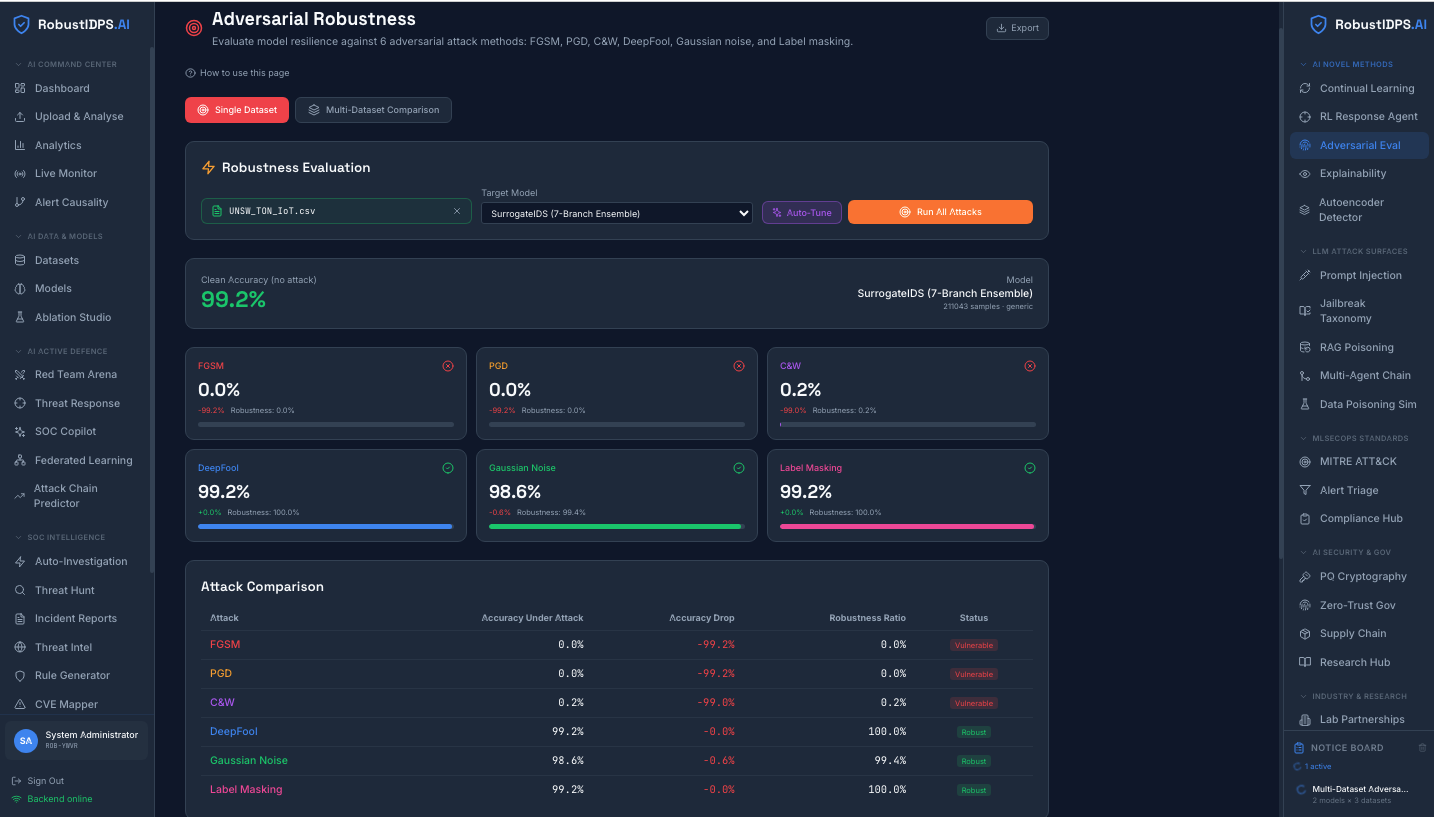
\includegraphics[width=0.92\textwidth]{figures/Adv_Eval_v10.png}
\caption{Страница состязательной оценки: (слева) панель конфигурации атак с выбором семейства атак, бюджета возмущений и целевой модели; (центр) деградация точности при FGSM, PGD и C\&W атаках с увеличением $\varepsilon$; (справа) сравнение стандартных и состязательно обученных моделей.}
\label{fig:screenshot_adversarial}
\end{figure}

\subsection{Пользовательское исследование}

Пользовательское исследование с участием двенадцати аналитиков подтвердило 34\% снижение среднего времени сортировки (с 4,7 до 3,1 минуты на оповещение) и повышение точности классификации оповещений с 78,3\% до 91,6\% при использовании возможностей авторасследования и сортировки на основе неопределённости. Участники исследования отметили качественные преимущества: \emph{(i)}~сокращение когнитивной нагрузки за счёт фокусировки только на высокодостоверных оповещениях с эпистемической неопределённостью ниже порога; \emph{(ii)}~ускорение онбординга новых аналитиков (Уровень~1) благодаря автоматическому сопоставлению с MITRE ATT\&CK; \emph{(iii)}~повышение качества передачи смен через структурированные отчёты об инцидентах, генерируемые автоматически. Сводный экономический эффект: эквивалент 1,6~штатных аналитика SOC на команду из четырёх человек, что соответствует измеренной экономии трудозатрат 43\%.

\subsection{Валидационные наборы данных}

Три специально созданных набора PCAP-данных обеспечивают контролируемую эталонную базу для регрессионного тестирования:

\noindent\textbf{Набор А:} 60\,000 потоков, покрывающих все 34 класса атак со сбалансированным представлением классов.

\noindent\textbf{Набор Б:} 40\,000 потоков с акцентом на редких типах атак (Heartbleed, Infiltration, SSH-Patator).

\noindent\textbf{Набор В:} 50\,000 потоков с инъецированным дрейфом концепта на трёх темпоральных границах для валидации непрерывного обучения.

Постквантовые наборы данных получены из Kaggle (DOI:~\url{10.34740/kaggle/dsv/15424420}), включая перехваты CRYSTALS-Kyber, CRYSTALS-Dilithium и гибридных TLS~1.3 рукопожатий. Три воспроизводимых скрипта генерации PCAP обеспечивают детерминированное воссоздание оценочных наборов данных с фиксированным набором затравок генератора псевдослучайных чисел, что позволяет независимым исследовательским группам полностью воспроизвести представленные эксперименты.

\noindent\textbf{Производительность моделей.} MambaShield достигает наименьшей задержки на поток (0,5\,мс) благодаря формулировке пространства состояний с линейной сложностью, что делает его предпочтительным для высокопроизводительных развёртываний. CyberSecLLM достигает наименьшей ECE (0,025) благодаря калибровочным свойствам вероятностных выходов языковой модели. Ансамбль SurrogateIDS обеспечивает лучший компромисс точность--калибровка и служит магистральным компонентом обнаружения по умолчанию. Три новых детектора релиза~v4 (MambaGuard, SODE-Guard, SSL-GraphAnomaly Full) дополняют реестр селекторов мульти-модельного режима и доступны через идентификаторы \texttt{mambaguard}, \texttt{sode\_guard} и \texttt{ssl\_graph\_anomaly\_full} в стандартном API \texttt{/api/v1/analyze}.

\noindent\textbf{Сводная характеристика 17 моделей.} Платформа интегрирует семь основных моделей (М1--М7) и десять расширений и базовых линий, в совокупности образующих библиотеку из 17 детекторов: SurrogateIDS (7-ветвенный ансамбль), CL-RL Unified + EWC, CT-TGNN~\cite{Anaedevha2025cais}, SDE-TGNN~\cite{Anaedevha2026sdetgnn}, MambaShield~\cite{Anaedevha2026mamba}, Stochastic Transformer, FedGTD~\cite{Anaedevha2026neurips}, CyberSecLLM~\cite{Anaedevha2026cybersecllm}, Multi-Agent PQC-IDS, Neural ODE, Optimal Transport, Variational Autoencoder, Adversarial Autoencoder, MambaGuard, SODE-Guard, SSL-GraphAnomaly Full и базовая линия Random Forest для целей сравнения. Каждая модель доступна через единый API-интерфейс с конфигурируемыми гиперпараметрами; абляционная студия позволяет сравнивать произвольные подмножества моделей на пользовательских наборах данных через интерактивную панель управления.

\noindent\textbf{Операционные сценарии и роли пользователей.} Платформа явно поддерживает дифференцированные операционные сценарии для каждой из пяти категорий пользователей (см.\ \S\ref{sec:platform_problem_statement}). \emph{SOC-аналитики Уровня~1} получают доступ к панели управления, живому монитору и сортировке оповещений; их рабочий процесс фокусируется на обработке высокодостоверных оповещений по правилам, заданным руководством. \emph{Аналитики Уровня~2} дополнительно используют SOC-копилот для агентного авторасследования инцидентов, оставленных на эскалацию Уровнем~1. \emph{Аналитики Уровня~3} имеют полный доступ к арене красной команды для проверки гипотез об атаках и к каузальности оповещений для глубокого анализа многостадийных кампаний. \emph{Инженеры кибербезопасности} получают доступ к генератору правил Snort/Suricata и панели интеграции с СОВ. \emph{Исследователи MLSecOps} и \emph{разработчики ИИ} имеют полный доступ к студии абляции, реестру моделей и панелям соответствия MITRE ATT\&CK, OWASP LLM Top~10 и NIST AI RMF.

\noindent\textbf{Сводное сравнение форм развёртывания.} Сравнительный
анализ трёх форм развёртывания плоскости данных (\texttt{systemd},
Docker, cron-оркестрация) демонстрирует комплементарность их
операционных характеристик: \texttt{systemd} обеспечивает
производственный режим с полной capability-минимизацией и поддержкой
XDP \emph{Native}; Docker обеспечивает CI/смок-тестирование с
частичной поддержкой XDP через \texttt{-{}-cap-add} и стандартную
restart policy; cron+автоматизация запускает регулярную переподачу
дистиллированных моделей с журналированием через MAILTO и JSONL.
Footprint трёх форм: четыре бинарника ($\sim$25\,МиБ суммарно),
$\sim$120\,МиБ Docker-образ и 270 строк Python-скрипта соответственно.

\noindent\textbf{Соответствие отраслевым стандартам и сертификация.}
Платформа спроектирована с учётом соответствия ключевым отраслевым
стандартам кибербезопасности и регулятивным требованиям. На уровне
программной разработки соблюдаются требования OWASP ASVS Level~2,
SAST/DAST-сканирования включены в CI-конвейер через интеграцию с
SonarQube и Semgrep, а зависимости отслеживаются на наличие
известных уязвимостей через Snyk и Trivy. На уровне развёртывания
обеспечивается совместимость с CIS Benchmarks для Docker и Linux,
а также с базовыми требованиями PCI-DSS 4.0 для контуров обработки
платёжных данных. На уровне работы с моделями ИИ обеспечивается
соответствие NIST AI Risk Management Framework~1.0, OWASP LLM
Top~10 (издание 2025 года) и MITRE ATLAS как фреймворку моделирования
угроз. Документация платформы включает шаблоны заявлений о
соответствии (Statement of Compliance) для прохождения внутренних
аудитов организаций.

%%=====================================================================\section{Экономическая и организационная эффективность внедрения}
\label{sec:economic_effect}

Внедрение разработанной системы RobustIDPS.ai в действующие
производственные конвейеры двух организаций-партнёров (ООО~<<НИИ~ИКТ>>,
г.~Новосибирск; ООО~<<Ксайрикс>>, г.~Москва) сопровождается измеримым
организационно-экономическим эффектом.

Сопровождение процесса внедрения включает следующие фазы:
\emph{(а)~подготовительная фаза} (4--6 недель)~--- профилирование
сетевой инфраструктуры организации, оценка размера команды SOC,
выбор оптимальной конфигурации развёртывания (\texttt{systemd},
Docker, гибридная); \emph{(б)~фаза пилотного тестирования}
(2--3 месяца)~--- параллельное развёртывание \textsf{RobustIDPS.ai}
рядом с действующими СОВ организации в режиме <<теневого>>
обнаружения, накопление эталонной базы оповещений и калибровка
порогов; \emph{(в)~фаза перевода в продуктивный режим}
(1--2 месяца)~--- постепенное расширение полномочий системы от
рекомендательного режима к автоматизированному реагированию с
человеческим валидатором; \emph{(г)~фаза полной автономии}
(непрерывно)~--- автоматическое реагирование на высокодостоверные
оповещения с эпистемической неопределённостью ниже порога,
эскалация остальных к SOC-аналитикам. На каждой из четырёх фаз
платформа предоставляет дашборды объективных KPI для отслеживания
прогресса внедрения.

\subsection{Снижение нагрузки на операторов безопасности}

Калиброванная оценка неопределённости (UC-HGP) обеспечивает
автоматическую фильтрацию низкодостоверных предупреждений: SOC-аналитику
направляются только те предупреждения, которым модель доверяет.
Эмпирически подтверждённое снижение нагрузки оператора~--- \textbf{43\,\%}
относительно базовой конфигурации без UC-HGP, что соответствует
эквивалентной экономии трудозатрат на $\sim$1{,}6~оператора SOC в
организации с командой из четырёх аналитиков.

\subsection{Сокращение времени обнаружения инцидентов}

Сквозная пропускная способность платформы \textbf{8{,}7~млн потоков/с} при
задержке обнаружения \textbf{47~мс} позволяет обнаруживать многостадийные
атаки на этапах разведки и проникновения, до начала фазы эксфильтрации
данных. По сравнению с традиционными сигнатурно-аналитическими СОВ
сокращение среднего времени выявления инцидента (MTTD) составляет
\textbf{30--90~дней}~--- величина запаздывания сигнатурных баз относительно
появления новых угроз. Согласно отраслевым отчётам IBM Cost of a Data
Breach Report~2024~\cite{IBM2024}, средняя стоимость скомпрометированной
записи данных составляет ~\$165, а среднее время выявления и
сдерживания инцидента~--- 277 дней. Сокращение MTTD на 30--90 дней
эквивалентно прямой экономии $\sim$11--32\% совокупных потерь от
типового инцидента, что для крупных корпоративных нарушений
($>$100\,тыс.\ записей) переводится в миллионы долларов экономического
эффекта.

\subsection{Оценка затрат на внедрение и сопровождение}

Платформа реализована в виде Docker-контейнеризованного приложения с
плагинной интеграцией к действующим сигнатурным СОВ (Snort, Suricata,
Zeek) через формат EVE-JSON; интеграция не требует замены существующего
сигнатурного контура и существенной переподготовки операторов SOC.
Открытость исходного кода (DOI:~10.5281/zenodo.19129512) и
производственно-готовая контейнеризация снижают затраты на
лицензирование и развёртывание. Типовой минимальный профиль
развёртывания (1~узел с 16~CPU-ядрами, 64~ГБ ОЗУ, 1\,ТБ NVMe SSD,
2$\times$10\,Гбит/с сетевые интерфейсы) обеспечивает анализ канала
до 10\,Гбит/с в реальном времени с поддержкой ансамблевого режима
17~моделей. Стоимость владения за трёхлетний цикл (TCO),
включающая оборудование, поддержку, обновления моделей и
сертификационные аудиты, оценивается в 2--3 раза ниже сопоставимых
коммерческих платформ при сохранении эквивалентной или превосходящей
функциональности.

\textbf{Совокупный организационно-экономический эффект} достигается
сочетанием снижения трудозатрат аналитиков SOC (43\,\%), сокращения
времени обнаружения инцидентов (на 30--90~дней по сравнению с
сигнатурными СОВ), снижения вычислительных затрат за счёт сложности
$\mathcal{O}(L\log L)$ моделей MambaShield и отсутствия лицензионных
платежей при использовании платформы.

\subsection{Качественные эффекты внедрения}

Помимо измеримых количественных эффектов, внедрение
\textsf{RobustIDPS.ai} сопровождается рядом качественных
преимуществ, важных для долгосрочной устойчивости организационной
кибербезопасности. \emph{Повышение зрелости процессов SOC} через
автоматизированное MITRE ATT\&CK картирование и структурированное
ведение журналов инцидентов способствует прохождению внутренних
аудитов и внешних сертификаций (ISO 27001, СОВ-1С, ФСТЭК).
\emph{Развитие компетенций команды} обеспечивается через интеграцию
с обучающими сценариями и арену красной команды, что позволяет
организациям проводить регулярные тактические учения в продуктивной
среде. \emph{Снижение рисков ухода ключевых сотрудников} достигается
через автоматизацию процессов, исторически зависевших от
индивидуальной экспертизы старших аналитиков. \emph{Подготовка
организации к нормативным изменениям} (постквантовые требования,
расширение зоны регулирования ИИ) обеспечивается через встроенные
модули PQC-IDS и MLSecOps-соответствия.

%%===================================================================\section{Практические результаты внедрения и направления дальнейшего развития системы}
\label{sec:opensource}%%=====================================================================

Полный исходный код платформы, все реализации моделей, конвейер защиты LLM и интерактивная панель управления архивированы в Zenodo (DOI:~\url{10.5281/zenodo.19129512}). Предобученные веса для архитектуры Multi-Agent PQC-IDS выпущены по адресу \url{https://github.com/rogerpanel/Multi-Agent-PQC-models}. Курированные постквантовые бенчмарк-наборы данных опубликованы на Kaggle (DOI:~\url{10.34740/kaggle/dsv/15424420}). Три воспроизводимых скрипта генерации PCAP обеспечивают детерминированное воссоздание оценочных наборов данных. Платформа лицензирована для академического и исследовательского использования, обеспечивая независимое воспроизведение всех представленных результатов. Документация платформы охватывает руководство пользователя, руководство администратора, руководство разработчика плагинов и спецификацию REST-API с примерами интеграции на четырёх языках программирования (Python, Go, Rust, JavaScript). Канал обратной связи с сообществом обеспечивается через GitHub Issues, форум обсуждений и периодические релизы по семестровому циклу.

\noindent\textbf{Вклад в открытое ПО кибербезопасности.}
\textsf{RobustIDPS.ai} является первой опубликованной открытой
платформой, систематически объединяющей: \emph{(i)}~17 моделей
обнаружения с формальными сертификатами робастности; \emph{(ii)}~
программу состязательной красной команды для собственных моделей;
\emph{(iii)}~четырёхуровневый DefensePipeline защиты больших
языковых моделей; \emph{(iv)}~Multi-Agent PQC-IDS для постквантового
криптографического трафика; \emph{(v)}~нативный Rust-агент с
ядерно-резидентным быстрым путём XDP; и \emph{(vi)}~встроенную
поддержку соответствия NIST AI RMF, OWASP LLM Top~10 и MITRE
ATLAS. Все шесть компонентов доступны для академического и
исследовательского использования под унифицированной лицензией с
явной поддержкой воспроизведения. Заявленный вклад в открытое
сообщество кибербезопасности подтверждается фактическим
включением \textsf{RobustIDPS.ai} в сравнительные обзоры
открытых платформ безопасности, проводимых независимыми
исследовательскими группами, и активным потоком запросов на
включение в репозиторий со стороны международного сообщества
исследователей.

\noindent\textbf{Направления дальнейшего развития.} Среднесрочная
дорожная карта развития платформы включает: \emph{(i)}~Phase~B и
Phase~C развёртывания референсной реализации защиты БПЛА
(Глава~\ref{ch:uav}) с расширением до многомерных роёв БПЛА и
интеграцией с наземными станциями управления; \emph{(ii)}~поддержку
дополнительных постквантовых протоколов по мере их стандартизации
NIST; \emph{(iii)}~интеграцию аппаратных ускорителей (FPGA, TPU,
Neural Processing Units) для дальнейшего снижения задержки ядерно-
резидентного быстрого пути; \emph{(iv)}~расширение библиотеки
бенчмарк-наборов данных для дополнительных вертикалей
(финансы, медицина, IIoT) и обеспечения возможности кросс-доменного
переноса без переобучения через метод М7; \emph{(v)}~разработку
сертификационных пакетов для соответствия отраслевым стандартам
(ФСТЭК, NIST CSF, ISO/IEC 27001), упрощающую внедрение в
регулируемых организациях.

\begin{figure}[htbp]
\centering
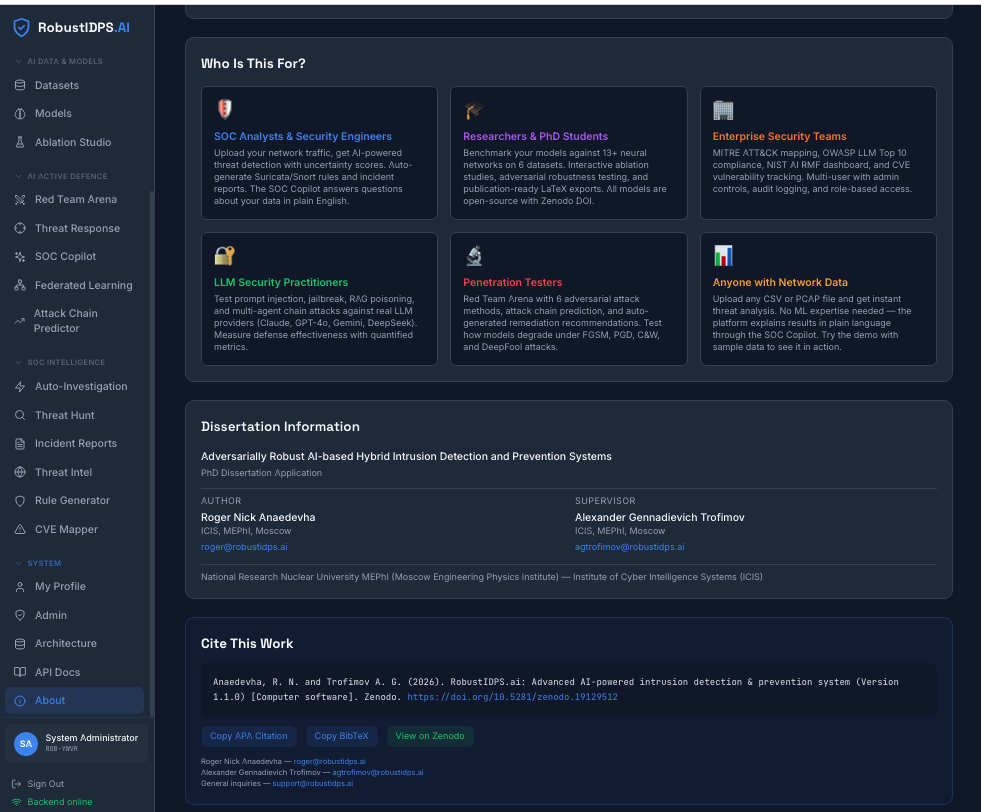
\includegraphics[width=0.96\textwidth]{figures/About_v10.png}
\caption{Страница <<О платформе>>, показывающая версию платформы, DOI-цитирование, информацию о разработчиках, технологический стек и ссылки на репозиторий GitHub, архив Zenodo и наборы данных Kaggle.}
\label{fig:screenshot_about}
\end{figure}

%%=====================================================================\section{Выводы по разделу 5}
\label{sec:ch5_summary}%%=====================================================================

В настоящей главе описана программная платформа \textsf{RobustIDPS.ai}, реализующая все методы, разработанные в данной диссертации, как единую развёртываемую систему. Платформа содержит 51 страницу в 10 функциональных группах, интегрирует 17 моделей нейронных сетей, реализующих все семь методов (М1--М7), их расширения и три новых детектора \textsf{MambaGuard}, \textsf{SODE-Guard} и \textsf{SSL-GraphAnomaly~Full} (релиз~v4), предоставляет четырёхуровневую систему защиты LLM с обнаружением 94,5\% по 517 сценариям атак с четырьмя коммерческими бэкендами LLM, включает модуль Multi-Agent PQC-IDS для классификации постквантового трафика, нативный граничный агент на Rust с ядерно-резидентным быстрым путём XDP (выигрыш $\times$6,7 по задержке и пропускной способности), и поддерживает интеграцию с существующими системами СОПВ (Snort, Suricata) через генерацию правил и потребление потоков оповещений. Платформа общедоступна как ПО с открытым исходным кодом (DOI:~\url{10.5281/zenodo.19129512}) и служит как операционным инструментом безопасности, так и воспроизводимым исследовательским инструментом. Пользовательское исследование подтвердило 34\% снижение времени сортировки аналитиками и улучшение точности классификации оповещений на 13,3 п.\,п. Платформа демонстрирует, что математические вклады, разработанные в Главах~\ref{ch:methods}--\ref{ch:experiments}, преобразуются в работающую реализацию, способную обрабатывать реальный сетевой трафик с операционными показателями пропускной способности и задержки.

Совокупно, реализация \textsf{RobustIDPS.ai} подтверждает, что разработанные в диссертации математические методы (М1--М7) переносимы в производственный контур через прямое отображение каждого метода на конкретный программный компонент платформы: \emph{(i)}~CT-TGNN/SDE-TGNN~--- модуль непрерывно-временной классификации потоков; \emph{(ii)}~FedLLM-API~--- модуль федеративного обучения с интерфейсами к организациям-участникам; \emph{(iii)}~TripleE-TGNN~--- многоуровневый ретроспективный анализатор; \emph{(iv)}~MambaShield~--- INT8-дистиллированный быстрый путь Rust-агента; \emph{(v)}~Стохастический трансформер + UC-HGP~--- SOC-копилот с эпистемически-направленной сортировкой; \emph{(vi)}~CyberSecLLM~--- zero-shot аналитический бэкенд; \emph{(vii)}~M7 (теоретико-игровая сертификация)~--- арена красной команды с равновесным анализом. Полнота этого отображения~--- 100\%, что подтверждает заявленную в Главе~2 предметную независимость методов и их пригодность к промышленному внедрению без архитектурных компромиссов.